\documentclass{article}
\usepackage[utf8]{inputenc}

\usepackage{amsthm}
\usepackage{amsmath}
\usepackage{amssymb}
\usepackage{xcolor}
\usepackage{tikz}

\theoremstyle{plain}
\newtheorem{thrm}{Théorème}[section]
\newtheorem{lem}[thrm]{Lemme}
\newtheorem{prop}[thrm]{Proposition}

\theoremstyle{remark}
\newtheorem{rem}[thrm]{Remarque}
\newtheorem{exmp}[thrm]{Exemple}

\theoremstyle{definition}
\newtheorem{defin}[thrm]{Définition}

\title{Apprentissage (Machine learning)}
\date{24 Septembre 2020}

\begin{document}

\maketitle

\section{Introduction}

L'apprentissage consiste à estimer des modèles à partir de données limitées, comme une liste d'exemples ou par des expériences. 
L'apprentissage contient plusieurs aspects :
\begin{itemize}
    \item Complexité
    \item Logique
    \item Algorithmique
    \item Statistique
\end{itemize}
Les méthodes d'apprentissage peuvent être regroupé dans les quatre catégories différentes suivantes :

\subsection{Apprentissage supervisé (supervised learning)}

L'ensemble $X=\{x_1,\cdots ,x_n\}$ est appelé le \emph{domaine}. L'ensemble $Y=\{y_1, \cdots , y_n \}$, s'il existe, est appelé l'\emph{ensemble d'étiquettage} (label set). Souvent on aura $Y=\{0,1\}$, et on parlera de classification.

Dans un apprentissage supervisé on a en données un domaine $X$ et un ensemble d'étiquettes $Y$. On cherche une fonction $h : X \rightarrow Y$ qui généralise les examples $(x,y)$ données.

INPUT : $(x_1,y_1),\cdots, (x_n, y_n)$

OUTPUT : $h : X\rightarrow Y$

\subsection{Apprentissage non supervisé (unsupervised learning)}

Dans un apprentissage non supervisé on a seulement le domaine $X$ en entrée sans étiquettes, et un entier $k$. Le but est de faire une partition de $X$ en $k$ classes.

INPUT : $x_1, \cdots , x_n$, $k\in \mathbb{N}$

OUTPUT : partition de $X$ en $k$ classes

\subsection{Apprentissage par récompense (Reinforcement Learning ou RL)}

Un ou plusieurs agents agissent sur un environnement (inconnu de base) et l'environnement répond aux actions des agents avec une récompense $r\in \mathbb{R}$. Le but est de choisir par essai-erreur les actions qui maximisent les récompenses. Contrairement à l'apprentissage supervisé et non supervisé on n'a pas de domaine et/ou ensembles d'étiquettage en INPUT/OUTPUT.

Exemple : AlphaGo

\subsection{Online Learning (apprentissage incrémentiel)}

L'apprentissage incrémentiel peut être supervisé ou non supervisé. Dans le cas supervisé, un couple supplémentaire $(x_i,y_i)$ est donné à chaque incrémentation $i$ et on en déduit une nouvelle hypothèse $h_i$.

On se concentrera par la suite sur l'apprentissage supervisé.


\section{Consistency model}

Soient $X$ un domaine, $Y$ un ensemble d'étiquettes et $\mathcal{H}\subset \{f : X \rightarrow Y \}$ un ensemble d'hypothèses.

Etant donné un échantillon (sample) $S=\{(x_i,y_i):i\in [1,|S|]\}$, on cherche une hypothèse $h\in \mathcal{H}$ tel que $h \models S$.

INPUT : un échantillon (sample) $S=\{(x_i,y_i) : i\in [1,|S|]\}$

OUTPUT : une hypothèse $h\in \mathcal{H}$ tel que $h \models S$ (c'est à dire $h(x_i)=y_i$ pour tout $i\in [1,|S|]$)

\begin{defin}
Un algorithme \textbf{apprend} $\mathcal{H}$ si pour tout échantillon $S$, l'algorithme retourne $h\models S$ avec $h\in \mathcal{H}$, ou ``il n'existe pas de $h\in \mathcal{H}$ tel que $h\models S$''.

De plus il est \textbf{efficace} s'il est en temps $poly(dim(x_i),|S|)$.
\end{defin}

Voici quelques exemples de consistency models (modèles de cohérence) :


\subsection{Formules conjonctives}

$X=\{0,1\}^n$, $n\in \mathbb{N}$,\\
$Y=\{0,1\}$\\
$\mathcal{H}_{FC}=\{\phi = \bigwedge_{p\in X_1} p \land \bigwedge_{p\in X_2} \neg p : X_1, X_2 \subseteq [1,n]\}$

Par exemple pour une dimension $n=4$ on a $\mathcal{H}=\{p_1, p_2, p_1\land \neg p_2, p_1\land p_2\land p_3\land p_4, p_4\land\neg p_3, \cdots \}$. Soit un échantillon $S=\{(x_1,y_1),\cdots,(x_5,y_5)\}$ définit comme suit :

\begin{center}
\begin{tabular}{ | c | c | c | c | c | c || c | c |  } 
    \hline
    & $p_1$ & $p_2$ & $p_3$ & $p_4$ & $p_5$ && \\
    \hline
    $x_1=$ & 0 & 1 & 0 & 1 & 1 & $y_1=$ & 1\\
    \hline
    $x_2=$ & 0 & 1 & 1 & 1 & 0 & $y_2=$ & 1\\
    \hline
    $x_3=$ & 0 & 1 & 1 & 0 & 1 & $y_3=$ & 0\\
    \hline
    $x_4=$ & 1 & 0 & 1 & 1 & 0 & $y_4=$ & 0\\
    \hline
    $x_5=$ & 0 & 0 & 0 & 1 & 1 & $y_5=$ & 0\\
    \hline
\end{tabular}
\end{center}

Soit $\phi=p_2\land p_4$, on a $x_1\models\phi$, $x_2\models\phi$, $x_3\not\models\phi$, $x_4\not\models\phi$, et $x_5\not\models\phi$, donc $S\models \phi$.

Voici une méthode pour trouver $\phi\in\mathcal{H}$ tel que $S\models \phi$ :

\begin{enumerate}
    \item On part de la plus longue formule $\phi = \bigwedge_{p\in X} p \land \bigwedge_{p\in X} \neg p$,
    \item puis, pour chaque $x_i$ tels que $y_i=1$, on enlève les $p_j$ tels que $x_{i,j}=0$ et les $\neg p_j$ tels que $x_{i,j}=1$,
    \item si $S\models \phi$, retourner $\phi$,
    \item sinon, retourner ``il n'y a pas de $\phi$''.
\end{enumerate}
Cet algorithme est de complexité $O(n|S|)$.

Dans le cas de l'exemple, on obtient :\\
$\phi = \textcolor{green}{p_1} \land \neg p_1 \land p_2 \land \textcolor{green}{\neg p_2} \land \textcolor{green}{p_3} \land \neg p_3 \land p_4 \land \textcolor{green}{\neg p_4} \land p_5 \land \textcolor{green}{\neg p_5}$\\
$\phi = \phantom{p_1} \land \neg p_1 \land p_2 \land \phantom{\neg p_2} \land \phantom{p_3} \land \textcolor{red}{\neg p_3} \land p_4 \land \phantom{\neg p_4} \land \textcolor{red}{p_5} \land \phantom{\neg p_5}$\\
$\phi = \neg p_1 \land p_2 \land p_4$

$\mathcal{H}$ est donc apprenable efficacement.

\subsection{Dysjunctive Normal Form (DNF)}

$X=\{0,1\}^n$, $n\in \mathbb{N}$,\\
$Y=\{0,1\}$\\
$\mathcal{H}_{DNF}=\{\phi = \bigvee_{i=1}^k C_i : C_i=\bigwedge_{p\in X_i} \pm p, X_i\subseteq X\}$

Par exemple pour une dimension $n=3$ on a $(p_1\land \neg p_2)\lor (p_3\land p_2)\in \mathcal{H}$. Remarquons que $\mathcal{H}_{FC}\subset\mathcal{H}_{DNF}$. Par ailleurs, pour $S=\{(x_i,y_i) : i\in [1,|S|]\}$ on obtient facilement une formule $\phi = \bigvee_{\{i:y_i=1\}} (\bigwedge_{\{j:x_{i,j}=1\}} p \land \bigwedge_{\{j:x_{i,j}=0\}} \neg p)$ tel que $S\models \phi$.

Avec l'échantillon $S$ décrit précédemment on obtient :

\begin{centering}
$\phi = (\neg p_1\land p_2\land\neg p_3\land p_4\land p_5)$\\
$\lor$\\
$\phantom{\phi =}(\neg p_1\land\neg p_2\land p_3\land p_4\land\neg p_5)$\\
\end{centering}

$\mathcal{H}$ est trivialement apprenable.

\subsection{3-Dysjunctive Normal Form (3-DNF)}

$X=\{0,1\}^n$, $n\in \mathbb{N}$,\\
$Y=\{0,1\}$\\
$\mathcal{H}_3=\{\phi = C_1\lor C_2\lor C_3 : C_i=\bigwedge_{p\in X_i} \pm p, X_i\subseteq X\}$

On va montrer que $\mathcal{H}_3$ n'est pas apprenable efficacement en montrant l'hypothèse cohérente suivante :

\'Etant donné un graphe $G$, on peut construire un échantillon $S=\{(x_i,y_i)\}$ tel que $G$ est 3-coloriable si et seulement si il existe $\phi\in\mathcal{H}_3$, tel que $S\models\phi$.

Le problème de 3-colorabilité est défini comme suit :

INPUT : un graphe $G$

OUTPUT : Est-ce qu'il existe une coloration $c : V \rightarrow \{R,V,B\}$, tel que $\forall e=(u,v)\in E$, $c(u)\neq c(v)$ ?

Par exemple, le graphe à $n=5$ et $m=7$ arêtes sommets suivant est 3-coloriable :

\begin{figure}[!h]
\centering
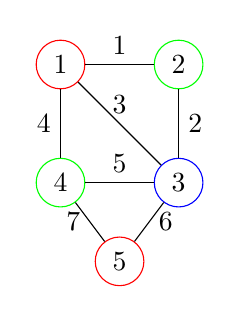
\begin{tikzpicture}
    \node[shape=circle,draw=red] (1) at (0,0) {1};
    \node[shape=circle,draw=green] (2) at (1.5,0) {2};
    \node[shape=circle,draw=blue] (3) at (1.5,-1.5) {3};
    \node[shape=circle,draw=green] (4) at (0,-1.5) {4};
    \node[shape=circle,draw=red] (5) at (0.75,-2.5) {5};
    
    \path[] (1) edge node[above] {1} (2);
    \path[] (2) edge node[right] {2} (3);
    \path[] (3) edge node[above] {5} (4);
    \path[] (4) edge node[left] {7} (5);
    \path[] (1) edge node[left] {4} (4);
    \path[] (1) edge node[above] {3} (3);
    \path[] (5) edge node[right] {6} (3);
\end{tikzpicture}
\end{figure}

Et on peut construire un échantillon\\
$S=\{(v_1,y_1),\cdots,(v_n,y_n),(e_1,y_{n+1}),\cdots,(e_m,y_{n+m})\}$ de dimension $n$ définit par :\\
- $y_i=1$ pour $i\leq n$, et $y_i=0$ sinon,\\
- $v_{i,i}=1$ et $v_{i,j}=0$ pour tout $i\neq j$,\\
- $e_{i,j}=1$ si et seulement si l'arête $i$ est incidente au sommet $j$.

\begin{center}
\begin{tabular}{ | c | c | c | c | c | c || c |  } 
    \hline
    & $p_1$ & $p_2$ & $p_3$ & $p_4$ & $p_5$ & y \\
    \hline
    $v_1=$ & 1 & 0 & 0 & 0 & 0 & 1\\
    \hline
    $v_2=$ & 0 & 1 & 0 & 0 & 0 & 1\\
    \hline
    $v_3=$ & 0 & 0 & 1 & 0 & 0 & 1\\
    \hline
    $v_4=$ & 0 & 0 & 0 & 1 & 0 & 1\\
    \hline
    $v_5=$ & 0 & 0 & 0 & 0 & 1 & 1\\
    \hline
    \hline
    $e_1=$ & 1 & 1 & 0 & 0 & 0 & 0\\
    \hline
    $e_2=$ & 0 & 1 & 1 & 0 & 0 & 0\\
    \hline
    $e_3=$ & 1 & 0 & 1 & 0 & 0 & 0\\
    \hline
    $e_4=$ & 1 & 0 & 0 & 1 & 0 & 0\\
    \hline
    $e_5=$ & 0 & 0 & 1 & 1 & 0 & 0\\
    \hline
    $e_6=$ & 0 & 0 & 1 & 0 & 1 & 0\\
    \hline
    $e_7=$ & 0 & 0 & 0 & 1 & 1 & 0\\
    \hline
\end{tabular}
\end{center}

\begin{proof}[Preuve]
1. $\Rightarrow$ : Supposons que $G$ est 3-coloriable et soit $c : V\rightarrow \{\textcolor{red}{R},\textcolor{green}{V},\textcolor{blue}{B}\}$ une coloration de $G$. Construisons $\phi=C_R\lor C_V\lor C_B$ tel que $S\models\phi$.\\
$C_R$ doit être satisfaite par $v_1$ et $v_5$ : $C_R=\neg p_2\land \neg p_3\land\neg p_4$. Comme les sommets 1 et 5 dans $G$ sont de même couleur, ils n'ont pas d'arête commune, donc pour tout $i$ on a $e_i \not\models \phi$. De même, on a $C_V=\neg p_1\land \neg p_3\land \neg p_5$ et $C_B=\neg p_1\land \neg p_2 \land \neg p_4 \land \neg p_5$.

2. $\Leftarrow$ : Supposons qu'il existe une formule $\phi=C_V\lor C_R\lor C_B$ tel que $S\models \phi$. Alors $G$ est bien 3-coloriable.
\end{proof}

Notons que dans le modèle de cohérence on assure que tout les $x_i$ tel que $y_i=1$ sont vrais et tout les $x_i$ tel que $y_i=0$ sont faux, hors on a plus de chance de généraliser avec une marge d'erreur, c'est à dire si on autorise quelques couples de l'échantillons à ne pas satisfaire l'hypothèse.

\section{PAC model}

\end{document}
